\chapter{Fritzing}
\label{chap:fritzing}

%%%%%%%%%%%%%%%%%%%%%%%%%%%%%%%%%%%%%%%%%%%%%%%%%%%%%%%%%%%%%%%%%%%%%%%%%%%%%%%%
% Objetivo: Exponer la herramienta Fritzing                                    %
%%%%%%%%%%%%%%%%%%%%%%%%%%%%%%%%%%%%%%%%%%%%%%%%%%%%%%%%%%%%%%%%%%%%%%%%%%%%%%%%

\lettrine{N}{este} apéndice exponse todo o relacionado coa ferramenta de deseño
hardware \textit{Fritzing}. \\

\textbf{Fritzing} \cite{Fritzing} é unha iniciativa software open source que
busca axudar a deseñadores e artistas a pasar de prototipos a productos finais.
Foi desenvolvido pola \textit{University of Applied Sciences of Potsdam}.

\section{Obxectivos}

O software creouse seguindo o espírito de Processing e Arduino e permite que un
deseñador, artista, invertigador ou afeccionado documente os seus prototipos
baseados en Arduino e cree un esquema dun PCB para a súa fabricación. O sitio
web \cite{Fritzing} permite compartir e discutir borradores e experiencias así
coma reducir os costes de fabricación. \\

Fritzing pode ser visto como unha ferramenta de automatizado de deseño
electrónico (EDA) para non enxeñeiros. \\

As imaxes dos compoñentes electrónicos distribúense baixo licencia CC-BY-SA,
que será tamén a licencia de calquera vista do resultado xerado.

\section{Interface de usuario}

Fritzing presenta unha interface fácil de usar para un fluxo de traballo rápido
e fácil. \\

 \subsection{Seccións}

 Consta principalmente de catro seccións (figura \ref{figura:FritzingBB}):

 \begin{itemize}
  \item Área de traballo: é a zona onde se montará o circuíto.
  \item Partes ou pezas: amosa a base de datos de pezas dispoñibles.
  \item Inspector de peza: amosa os datos concretos dunha peza.
  \item Navegador de vistas: permite cambiar entre as tres vistas principais.
 \end{itemize}

 \begin{figure}[htbp]
  \centering
  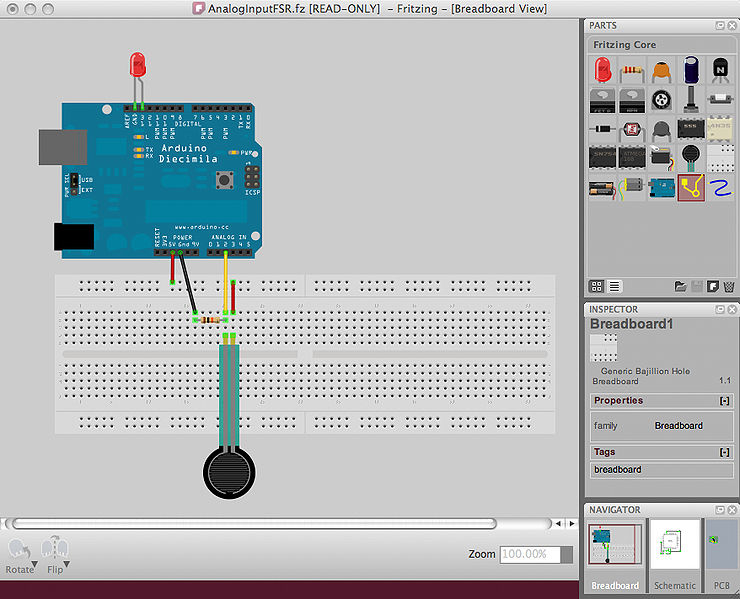
\includegraphics[scale=0.3,keepaspectratio=true]{./imagenes/fritzing-bb.jpg}
  % fritzing-bb.jpg: 740x599 pixel, 72dpi, 26.11x21.13 cm, bb=0 0 740 599
  \caption{Fritzing: vista de prototipado}
  \label{figura:FritzingBB}
 \end{figure}

 \subsection{Vistas}

 Consta de tres vistas principais:

 \begin{itemize}
  \item Vista de prototipado: amosa a vista real dos compoñentes.
  \item Vista esquemática: amosa o esquema de conexión.
  \item Vista de PCB: amosa cómo quedaría o PCB.
 \end{itemize}

 \begin{figure}
  \centering
  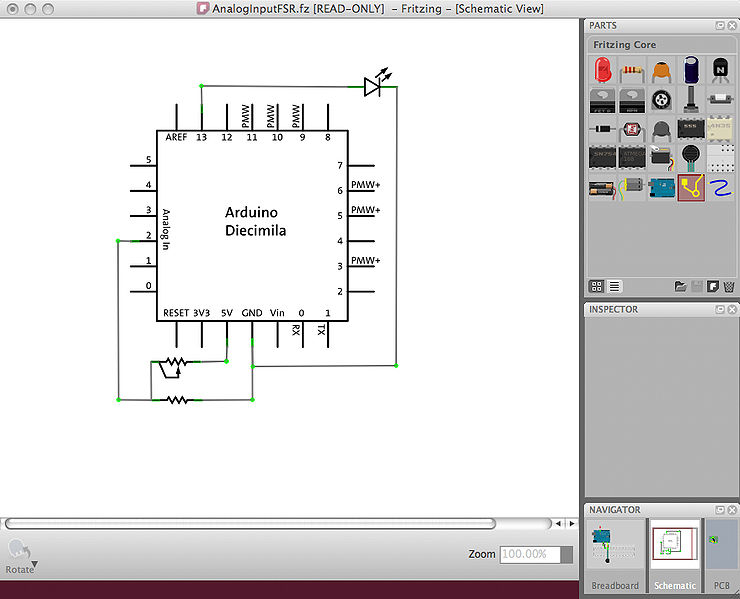
\includegraphics[scale=0.3,keepaspectratio=true]{./imagenes/fritzing-esquema.jpg}
  % fritzing-esquema.jpg: 740x599 pixel, 72dpi, 26.11x21.13 cm, bb=0 0 740 599
  \caption{Fritzing: vista esquemática}
  \label{figura:FritzingEsquema}
 \end{figure}

 \begin{figure}
  \centering
  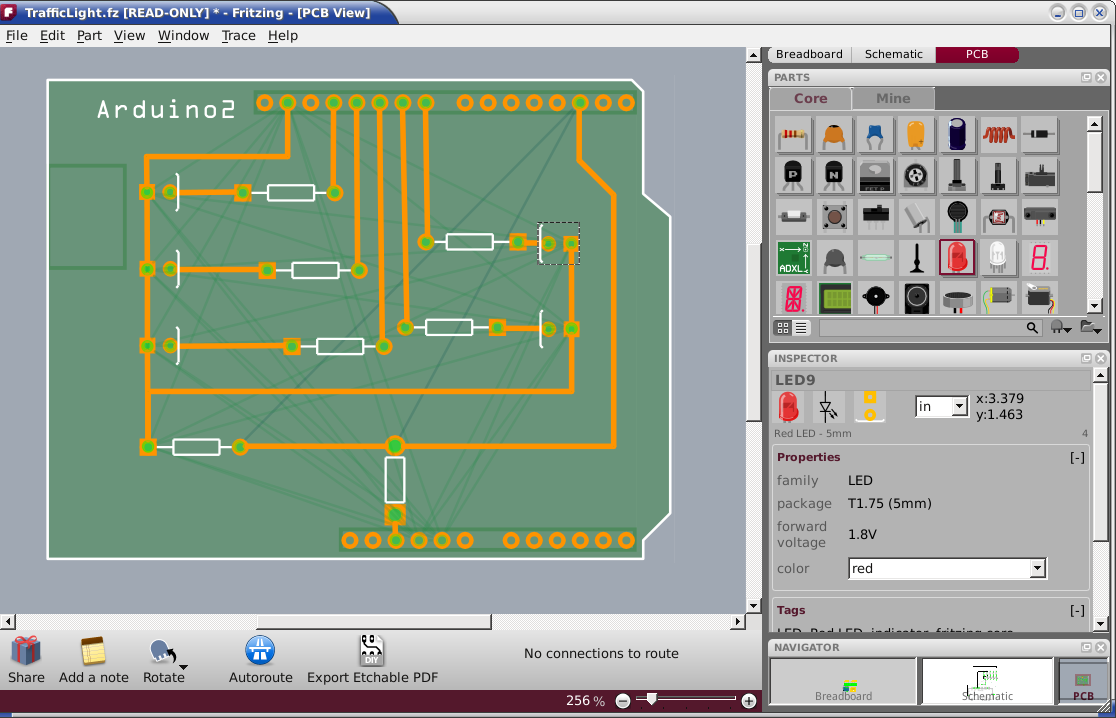
\includegraphics[scale=0.3,keepaspectratio=true]{./imagenes/fritzing-pcb.png}
  % fritzing-pcb.png: 1116x718 pixel, 95dpi, 29.84x19.20 cm, bb=0 0 846 544
  \caption{Fritzing: vista de PCB}
  \label{figura:FritzingPCB}
 \end{figure}

